
\chapter{Resultate der Arbeit}
\subfile{./sections/results/patterns}
\subfile{./sections/results/application}
\subfile{./sections/results/criterias}

\section{Diskussion der Ergebnisse des Vergleichs der Alternativen}
Der Architekt wertet die Ergebnisse der Arbeit nicht. Die Alternativen haben alle Chancen und Risiken.

Der Architekt wird im weiteren Verlauf eine Diskussion führen über ausgewählte Erkenntnisse aus dem Vergleich der Alternativen.

\subsection{Ausarbeitungszeit der Prototypen}
Die \marg{Backend-Komposition} Ausarbeitungszeit der Prototypen zeigte eine klare Reihenfolge  von der Komplexität auf. Die \textit{Backend-Komposition} ist die einfachste Komposition zum implementieren. 

Statt die Daten aus der Datenbank zu laden, werden die Daten von einem Hintergrundservice geladen. Die Restlichen Arbeitsschritte, Daten aus Object Tree extrahieren und Template rendern sind analog zu lokalem Datenrendering.

Die \marg{Portal-Komposition} Portal-Komposition ist die zweitschwierigste Komposition zum implementieren. Die Fragmenteinbindung von externen Services in Thymeleaf stellte ein schwieriges und fehleranfälliges Unterfangen dar. Dies führte zu langer Fehlersuche.

Die \marg{Frontend-Komposition} Frontend-Komposition war die schwierigste Komposition, da es sehr viele Technologien beinhaltete. Über den Server musste CORS dektiviert werden und auf dem Client musste ich ReactJS lernen. Weil React keine HTTP-Bibliothek beinhaltet, musste ich noch einen Adapter \cite{Gamma1995} schreiben um die JQuery\footnote{\url{https://jquery.com/}} Bibliothek einzubinden. 

\subsection{Unterbrechungsfreie Aktualisierbarkeit: Kann das Microfrontend zusammen mit dem Microservice ausgetauscht werden?}\label{chap:results:main:Aktualisierbarkeit}

Mit der \marg{Portal Komposition} \textit{Portal Komposition} konnte gezeigt werden, dass ein Frontend auf dem Applikationsserver abgelegt werden kann. Das Frontend kann mit dem Austausch des Applikationsservers in einem Schritt aktualisiert werden. 

Weil bei der Portal Komposition die \ac{HTML}-Dokumente lokal gerendert werden, ist eine Aktualisierung des Domain-Models nur die Aktualisierung des Applikationsservers nötig.

Das \ac{UI} der \marg{Backend Komposition} Backend Komposition kann nicht mit der Aktualisierung des Applikationsservers ersetzt werden. Bei dieser Alternative muss der Webserver ersetzt werden. 

Solange das Übertragungsprotokoll nicht ändert, muss der Applikationsserver nicht ersetzt werden. Wenn die Domain-Model der Applikation ändert muss der Applikationsserver, der Webserver und das Übetragungsprotokoll zwischen den zwei Tiers aktualisiert werden.

Die Meinung \marg{Web Compontents} des Autors ist, dass mit der Nutzung von WebComponents eine Microfrontent-Architektur im Browser aufgebaut werden kann. Dann können WebComponents auf den Applikationsserver abgelegt werden. Durch den Einsatz von \textit{HTML Imports}\cite{w3cHtmlImports} kann das HTML-Dokument auf die Services aufgeteilt werden und durch den Browser zusammengefügt werden.

Die WebComponents Technologie ist zur Zeit der Abgabe dieser Arbeit experimentell und wenig unterstützt durch die Browserlandschaft. Dies zeigte eine \textit{caniuse}\footnote{\url{https://caniuse.com/\#search=web\%20components}} Abfrage. Die Auswertung der Brwoserunterstützung aller Spezifikationen zur Technologie ist unter \ref{fig:results:main:WebComponents}  ersichtlich. Chrome und seine Derivate implementieren die Spezifikation schon. Andere Browserhersteller sind noch nicht soweit, dass diese Technologie produktiv einsetzbar ist.

\begin{figure}
    \centering
    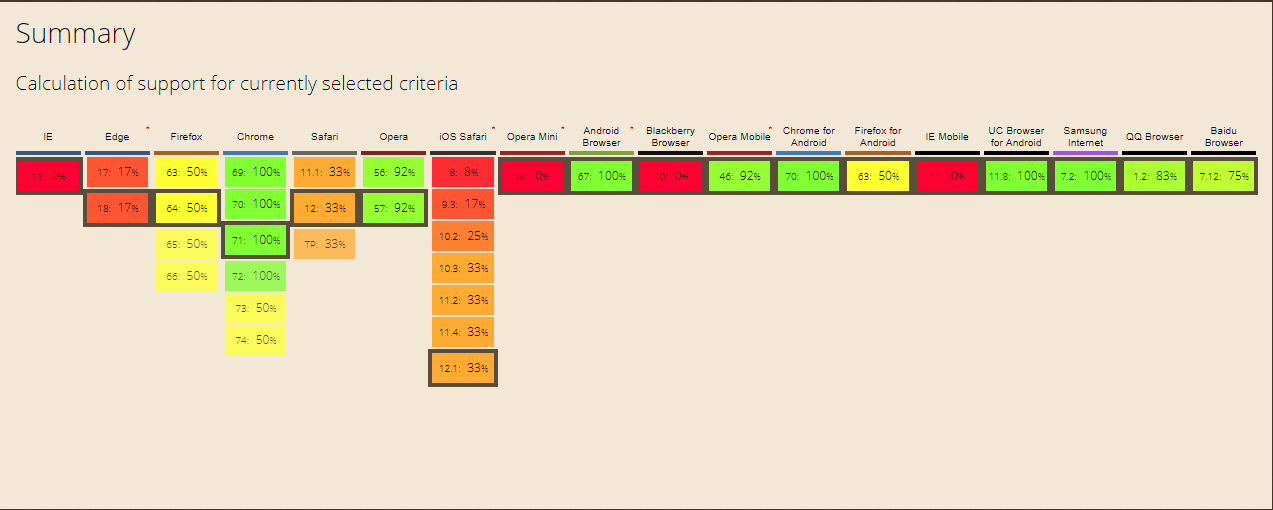
\includegraphics[width=\textwidth]{sections/results/WebComponents.png}
    \caption{caniuse Abfrage für WebComponents}
    \label{fig:results:main:WebComponents}
\end{figure}

Der Architekt \marg{Zusammenfassung} schätzt die Einfachheit der Portal Komposition. Die Backend Komposition hat gute Trennung der Belange. Der Architekt geht davon aus, dass die Frontend-Komposition mit WebComponents in der Zukunft der Standard für Microfrontends wird. Bis dahin, sind alle Alternativen gute Lösungen.

\subsection{Die Microfrontend Architektur darf nicht die Unabhängigkeit der Microservices erweichen}

Diese \marg{Aufgetretene Risiken} Anforderung konnte die Beispielapplikation nicht vollständig erfüllen. Der Entwickler konnte zeigen, dass der Code aller Implementationsformen voneinander unabhängig ist. Aufgrund von Projektbeschränkungen konnte der Architekt die Integrationen nicht in verschiedene Services auftrennen um eine Three-Tier-Architektur aufzubauen.

Eine \marg{Chancen} weiterer Anknüpfungspunkt für eine Folgearbeit ist die Analyse und prototypische Implementation von WebComponents. \cite{mdnWebComponents}

Ich \marg{Zusammenfassung} konnte im Zuge dieser Arbeit die Möglichkeit aufzeigen, dass es möglich ist alle Kompositionsalternativen aufzutrennen und überlasse die Auftrennung einer Folgearbeit.

\subsection{Erkenntnisse über mögliche Technologien}

Für den Browser gibt es die \marg{WebComponents} WebComponents-Technologie. \cite{mdnWebComponents} Für die Diskussion der Chancen und Risiken von WebComponents siehe Sektion \ref{chap:results:main:Aktualisierbarkeit}.

Die Technologie \marg{server-side includes} \ac{SSI}\footnote{\url{https://www.w3.org/Jigsaw/Doc/User/SSI.html}} wird im Zusammenhang mit \ac{HTML}-Fragmentenkomposition häufig erwähnt. Die Konvention erlaubt unter Apache Server\footnote{\url{https://httpd.apache.org/}} das Zusammenfügen von Websitenteile verschiedener Applikationen. Diese Technologie steht unter Spring nicht zur Vefügung und wurde deshalb in dieser Arbeit nicht weiter untersucht.

Die Technologie \marg{edge-side includes} \ac{ESI}\footnote{\url{https://www.akamai.com/fr/fr/support/esi.jsp}} kann verwendet werden um Inhalte verschiedener URL's auf einem Proxy-Server in ein gemeinsames \ac{HTML}-Dokument zusammen zu führen. Diese Technologie wird stark von Akamai\footnote{\url{www.akamai.com}} und fastly\footnote{\url{https://www.fastly.com/}} genutzt um Bilder und weitere Cache Inhalte in Kundenseiten zu integrieren.\cite{FastlyESI} Weil die Proxy-Variante nicht weiterverfolgt wurde ist diese Technologie nicht näher betrachtet worden in der Arbeit.